\section{系统测试}

系统测试是将需测试的软件,作为整个基于计算机系统的一个元素,与计算机硬件、外设、某些支持软件、数据和人员等其他系统元素及环境结合在一起测试。 在实际运行(使用)环境下,对计算机系统进行一系列的组装测试和确认测试。系统测试的目的在于通过与系统的需求定义作比较,发现软件与系统定义不符合或与之矛盾的地方。

\subsection{测试目标}

\begin{enumerate}
	\item 查看系统中是否有逻辑错误以及逻辑冲突。发现系统中存在的问题,完善系统的设计逻辑。确保系统逻辑的稳定性,避免系统死锁等情况。
	\item 确立各个子模块以及主模块之间的状况。保证集成之后系统各模块之间的良好配合。
	\item 优化系统设计,找出系统缺陷,保证系统更加符合软件工程,可以得到良好的再维护可能。
	\item 进行实际的数据测试,保证各个模块能够对数据进行正常的数据处理和响应。
\end{enumerate}

\subsection{测试方案}

首先对于系统的各个子模块进行代码审查,如用户登录验证模块,节点管理模块等。确保各个子模块之间的代码的健壮性和稳健性。另外,还需要进行功能性测试,确保功能正常,可以按照预期目标产生相应的结果。

设计测试方案如下:
 
1. 通过MQTT客户端与服务端进行通信,查看服务端能否介绍到相应数据。测试过程如下所示:
\begin{figure}[htbp]
	\centering
	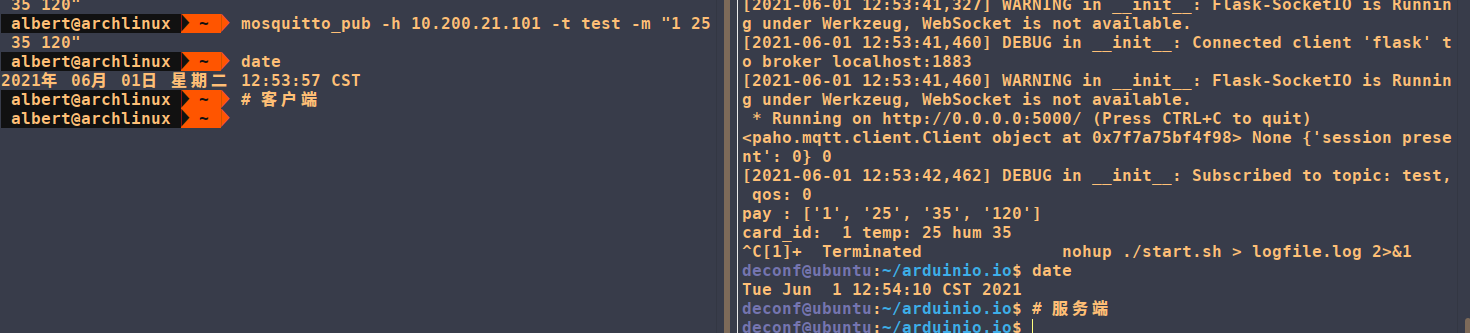
\includegraphics[width=0.85\linewidth]{figure/test-1}
	\caption{MQTT数据接受测试}
	\label{fig:6-1}
\end{figure}
如图\ref*{fig:6-1} 所示,MQTT服务器可以接收到相应的发送数据。

2. 检查MQTT服务器接收的数据是否存入到后端存储MySQL服务器中,测试过程如下所示:
\begin{figure}[htbp]
	\centering
	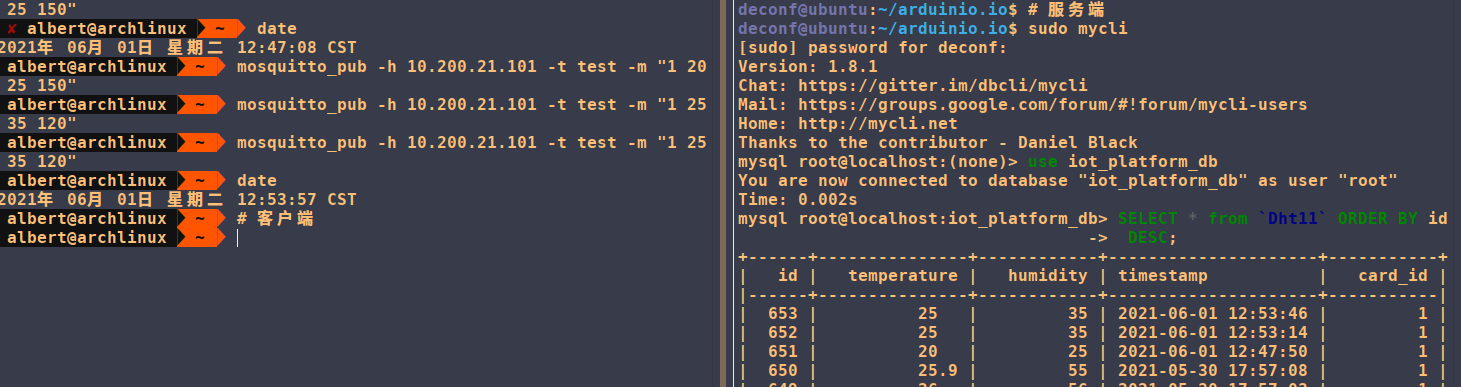
\includegraphics[width=0.85\linewidth]{figure/test-2}
	\caption{MQTT数据存储测试}
	\label{fig:6-2}
\end{figure}
如图\ref{fig:6-2} 通过时间戳可以判定数据已经接受并已经存储在后端MySQL服务器上。

3. 测试当数据超过设计相应的阈值,检查触发相应的警报模块,是否可以正常发送告警信息。
\begin{figure}[htbp]
	\centering
	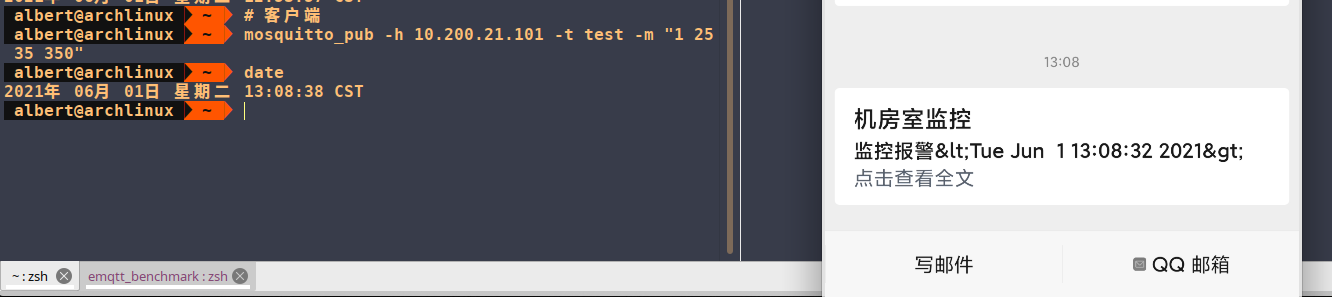
\includegraphics[width=0.85\linewidth]{figure/test-3}
	\caption{MQTT数据报警测试}
	\label{fig:6-3}
\end{figure}
如图\ref{fig:6-3}所示,在数据超过预设阈值之后,几乎可以同时收到相应的邮件告警信息。

\subsection{关于MQTT服务器高并发的测试}

\begin{table}[H]
	\centering
	\caption{测试环境配置}  %表格标题
	\begin{tabular}{ll} 
		\hline
		\hline
		核心硬件 & 型号 \\ 
		\hline
		CPU	& Intel Core i7 9xx (Nehalem Core i7, IBRS update) @ 6x 2.267GHz		\\
		RAM	& DDR3 1600MHz 4Gb \\
		HDD	& 40G \\
		\hline
		\hline
		核心软件 & 版本 \\ 
		\hline
		OS	& Ubuntu 18.04.5 LTS \\
		Python & v3.6.9 \\
		Flask & v1.0.3 \\
		mosquitto & v1.4.15 \\
		\hline
	\end{tabular}
\end{table}

此外,由于是分布式系统,那么对于系统的高并发测试也是必须进行的一个项目。服务器的高并发性能代表着服务器能容纳的节点数量以及可接入的客户端数量。代表之后可扩展的容量限制。

测试方案如下:

通过使用开源项目emqtt-bench模拟MQTT客户端与服务端进行通信,查看服务端的负载压力情况如下所示:


\begin{figure}[H]
	\centering
	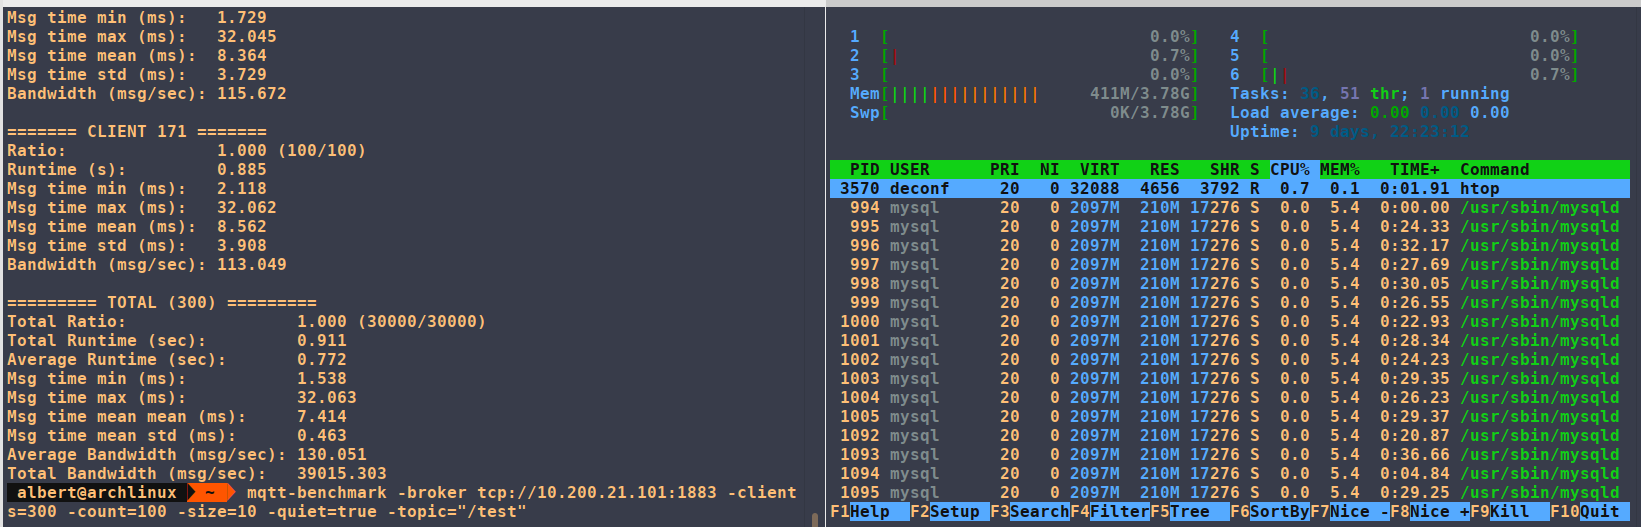
\includegraphics[width=0.85\linewidth]{figure/test-4}
	\caption{MQTT负载压力测试}
	\label{fig:6-4}
\end{figure}

如上图\ref{fig:6-4}在300个客户端同时订阅发布的情况下,得到了平均相应时间为0.772 ms
,最大响应时间为32.063ms,可以得出,系统可近似认为其为实时处理。
通过服务端的htop软件查看系统负债情况,发现MQTT服务端软件mosquitto几乎不占用负债情况。得益于MQTT协议的设计,在高并发的情况下,负载情况表现良好。